\documentclass[a4paper]{article}

\usepackage{graphicx}
\usepackage{amsmath}
\usepackage[margin=1in]{geometry}

\title{Classical internet applications
\newline Lab session: Booting 1}
\author{Anatoly Tykushin \small { MSIT-SNE a.tykushin@innopolis.ru}}

\begin{document}
\pagenumbering{arabic}
\maketitle
\tableofcontents 

\newpage
\section{Installation report}
During installation has been occurred a couple of arguing situations:

\begin{itemize}
\item Firstly, default boot devices priority wasn?t set correctly, that?s why PC didn?t boot via NIC (network interface controller) and didn?t get any IP address from DHCP server.
\item Secondly, you should configure this option: \newline \textbf{ Bios $ \rightarrow $ Advanced $ \to $ Option ROM launch $policy \to $ PXE option ROM $ \to $ UEFI only}
\item Thirdly, there were a couple of problems with GPT partiion took place. To solve it we had to delete old partitions and reallocate hard-disks. 
\end{itemize}

\section{Answering the questions after installation}
\subsection{Preboot Execution Environment}
\subsubsection{What is UEFI PXE booting?}
Unified Extensible Firmware Interface (UEFI) is a specification that defines a software interface between an operating system and platform firmware.  \newline
UEFI replaces the Basic Input/Output System (BIOS) firmware interface originally present in all IBM PC-compatible personal computers, with most UEFI firmware implementations providing legacy support for BIOS services. UEFI can support remote diagnostics and repair of computers, even with no operating system installed. \newline
UEFI has various booting mechanisms: from hard disk, cd, removable media and network. So, UEFI PXE is a PC's booting method, which serves a UEFI signed grub image (network image), loads the configuration in grub.cfg and boots the Linux kernel. 
\subsubsection{How does it work?}
PXE booting consists of 9 stages. They will be listed below:

\begin{description}
\item[Stage 1] PXE client sends DHCP Discover (port 67) including:
	\begin{itemize} 
		\item A tag for client identifier (UUID)
		\item A tag for the client UNDI version
		\item A tag for the client system architecture.
		\item A DHCP option 60, ClassID, set to \textbf{PXEClient:Arch:xxxxx:UNDI:yyyzzz}
	\end{itemize}
\item[Stage 2] On the stage 2 client gets DHCPOFFER message (port 68).
\item[Stage 3] Client records
	\begin{itemize} 
		\item The Client IP address (and other parameters) offered by a standard DHCP or BOOTP Service.
		\item The Boot Server list from the Boot Server field in the PXE tags from the DHCPOFFER.
		\item The Discovery Control Options (if provided).
		\item The Multicast Discovery IP address (if provided). 
	\end{itemize}
\item[Stage 4] Here comes the approval of client's API
\item[Stage 5] The client selects and discovers a Boot Server. This packet may be sent broadcast (port 67), multicast (port 4011), or unicast (port 4011) depending on discovery control options included in the previous DHCPOFFER containing the PXE service extension tags. It is DHCPREQUEST and contains the following: 
	\begin{itemize} 
		\item The IP address assigned to the client from a DHCP Service.
		\item A tag for client identifier (UUID)
		\item A tag for the client UNDI version.
		\item A tag for the client system architecture. 
		\item A DHCP option 60, ClassID, set to \textbf{PXEClient:Arch:xxxxx:UNDI:yyyzzz}
		\item The BootServer type in a PXE option field
	\end{itemize}
\item[Stage 6] The Boot Server unicasts a DHCPACK packet back to the client on the client source port. This reply packet contains: 
	\begin{itemize}
		\item Boot file name
		\item MTFTP configuration parameters
		\item Any other options the NBP requires before it can be successfully executed.
	\end{itemize}
\item[Stage 7] The client downloads the executable file using either standard TFTP (port69) or MTFTP (port assigned in Boot Server Ack packet). The file downloaded and the placement of the downloaded code in memory is dependent on the client?s CPU architecture. 
\item[Stage 8] The PXE client determines whether an authenticity test on the downloaded file is required. If the test is required, the client sends another DHCPREQUEST message to the boot server requesting a credentials file for the previously downloaded boot file, downloads the credentials via TFTP or MTFTP, and performs the authenticity test. 
\item[Stage 9] Finally, if the authenticity test succeeded or was not required, then the PXE client initiates execution of the downloaded code.
\end{description}

\subsubsection{How does it compare to booting from the hard disk or a CD?}
Booting from hard disk or a CD is a process of file name in the form \textbf{\textbackslash EFI\textbackslash BOOT\textbackslash BOOT\textbackslash \textless machine type short-name\textgreater .EFI} where machine type short- name defines a PE32+ image format architecture. Each file only contains one UEFI image type, and a system may support booting from one or more images types. In this case boot loader is already installed to the machine. 
Booting from PXE is the way to start disk-less computer using network card. PXElinux loader gets the linux image and delegates all management to it. After that linux asks server where is the root filesystem and then starts loading.



\subsection{GUID Partition Table}
\subsubsection{What is GPT?}
GUID Partition Table (GPT) is a standard for the layout of the partition table on a physical storage device, such as a hard disk drive or solid-state drive, using globally unique identifiers (GUID). Although it forms a part of the Unified Extensible Firmware Interface (UEFI) standard (Unified EFI Forum proposed replacement for the PC BIOS), it is also used on some BIOS systems because of the limitations of master boot record (MBR) partition tables, which use 32 bits for storing logical block addresses (LBA) and size information on a traditionally 512 byte disk sector.

\subsubsection{What is its layout?}
\begin{figure}[h!]
  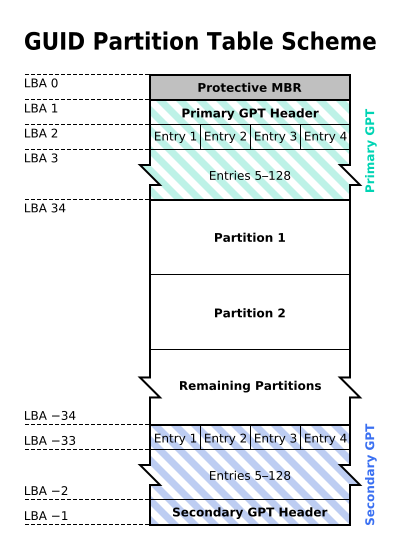
\includegraphics[width=8cm]{GPT.png}
  \caption{GUID Partition Table Scheme.}
  \centering
  \label{fig:gpt}
\end{figure}

Let's get more detailed view to the partition table scheme shown in figure \ref{fig:gpt}.
It contains:
\begin{itemize}
	\item Protective MBR (LBA 0)- for limited backward compatibility, the space of the legacy MBR is still reserved in the GPT specification, but it is now used in a way that prevents MBR-based disk utilities from misrecognizing and possibly overwriting GPT disks.
	\item Partition table header (LBA 1) -the partition table header defines the usable blocks on the disk. It also defines the number and size of the partition entries that make up the partition table. The EFI stipulates a minimum of 16,384 bytes be reserved for the partition table array, so there are 128 partition entries reserved, each 128 bytes long.
	\item Partition entries - partition entry array describe partitions, using 128 byte blocks per entry at a minimum. They contain GUID (globally unique identifier)
\end{itemize}


\subsubsection{What is the role of a partition table?}
A partition table is a table maintained on disk by the operating system describing the partitions on that disk. The terms partition table and partition map may be used generically to refer to other "formats" that divide a disk drive into partitions (GUID, APM, BSD).

\subsection{Gdisk utility}
\subsubsection{What is gdisk?}
Gdisk - Interactive GUID partition table (GPT) manipulator. A text-mode menu-driven program for creation and manipulation of partition tables. It will automatically convert an old-style Master Boot Record (MBR) partition table or BSD disklabel stored without an MBR carrier partition to the newer Globally Unique Identifier (GUID) Partition Table (GPT) format, or will load a GUID partition table.

\subsubsection{How does it work?}
Ordinarily, gdisk operates on disk device files, such as \textbf{\textit{/dev/sda}} or \textbf{\textit{/dev/hda}} under Linux, \textbf{\textit{/dev/disk0}} under Mac OS X, or \textbf{\textit{/dev/ad0}} or \textbf{\textit{/dev/da0}} under FreeBSD. The program can also operate on disk image files, which can be either copies of whole disks (made with dd, for instance) or raw disk images used by emulators such as QEMU or VMWare. Note that only raw disk images are supported; gdisk cannot work on compressed or other advanced disk image formats.
\subsubsection{What can you do with it?}
It also has the capability of transforming MBR partitions or BSD disk labels into GPT partitions. Like the original fdisk program, gdisk does not modify disk structures until you explicitly write them to disk, so you have a chance to decline your mistakes of partitioning. 
\begin{itemize}
	\item It can convert existing MBR- and BSD partitions to GPT format
	\item It works with GUID
	\item It creates hybrid (MBR+GPT) partitions 
   	\item Enables declining partition operations because of not straight recording to hard disks.
\end{itemize}

\subsection{What is Protective MBR and why is it in GPT?}
Protective MBR is for limited backward compatibility, the space of the legacy MBR is still reserved in the GPT specification. It is now used in a way that prevents MBR-based disk utilities from misrecognizing and possibly overwriting GPT disks. 

\section{Partition}
\subsection{Parsing GPT}
By using dd utility file containing protective MBR record and GPT was created.
Copy and dump the Protective MBR and GPT in hex format on your moodle account, and fully annotate the entries. This means you must describe the purpose of every field, and translate all fields that have a numerical value into human readable, decimal format. Result of parsing dump of protective MBR and GPT partition is shown in section \ref{subsec:gpt_parse}.
\subsubsection{At what byte index from the start of the disk do the real partition table entries start?}
GPT header starts from 0x200 (513th) byte (because of protective MBR?s length is 512 byte). There starts primary GPT header. Partition table begins at 1025th byte (offset = 512+512=1024 bytes)


\subsubsection{At what byte index would the partition table start if your server had a so-called ?4K native?
(4Kn) disk?}
In 4Kn technology eight 512-byte sectors become one 4Kb sector. In this case GPT Header will start at 8193rd byte (offset = 4096+4096 = 8192 bytes - they are used for protective mbr and gpt header, after them goes gpt parition table).

\subsection{FreeBSD partition question}
If you wanted to add a (1 + your table number) GiB FreeBSD ZFS partition, called �S3 (U+00D8
U+015A U+0033) to the table by hand, what values would you have ? to use for the entry (including the name) in the raw table on disk? Assume the disk is large enough to hold the extra partition. \newline \newline
Desired partition will start at 917.6 GiB, at the end of last partition(for Ubuntu). The answer will be shown in section \ref{subsec:freebsd}.

\newpage
\section{Parsing results}
\subsection{GPT parsing results}
\label{subsec:gpt_parse}
In this section we can see parsed file. Strings with 0's are missing because they doesn't have a semantic meaning. 
Dump of GPT is shown in table \ref{table:gptdump}.
\begin{table}[h!]
\begin{center}
  \begin{tabular}{ l | l | l }
    Offset & Value & ASCII form \\
    \hline
    	000001c0: & 00ee feff ff01 0000 00af 6d70 7400 0000 & ..........mpt... \\
    	000001d0: & 0000 0000 0000 0000 0000 0000 0000 0000 &  ................ \\
    	000001e0: & 0000 0000 0000 0000 0000 0000 0000 0000 & ................ \\
   	000001f0: & 0000 0000 0000 0000 0000 0000 0055 aa45 & .............U.E \\
    	00000200: & 4649 2050 4152 5400 0001 005c 0000 00e2 & FI PART...../... \\
    	00000210: & c54d a700 0000 0001 0000 0000 0000 00af & .M..............\\
    	00000220: & 6d70 7400 0000 0022 0000 0000 0000 008e & mpt...."........ \\
    	00000230: & 6d70 7400 0000 00b4 2698 34e3 3bb5 4dae & mpt......M.  \\
    	00000240: & 8576 c2a5 cb9d 8702 0000 0000 0000 0080 &  .v.............. \\
    	00000250: & 0000 0080 0000 0058 c507 ca00 0000 0000 & ........X...... \\
    	000003f0: & 0000 0000 0000 0000 0000 0000 0000 0028  & ...............( \\
	00000400: & 732a c11f f8d2 11ba 4b00 a0c9 3ec9 3b7c  & s*......K...>.;| \\
	00000410: & b304 539d c76c 43bb 2085 8571 70c8 d800  &..S..lC. ..qp... \\
	00000420: & 0800 0000 0000 00ff 0710 0000 0000 0000  & ................ \\
	00000430: & 0000 0000 0000 0045 0046 0049 0020 0053  &.......E.F.I. .S \\
	00000440: & 0079 0073 0074 0065 006d 0020 0050 0061  & .y.s.t.e.m. .P.a \\
	00000450: & 0072 0074 0069 0074 0069 006f 006e 0000  & .r.t.i.t.i.o.n.. \\
	00000460: & 0000 0000 0000 0000 0000 0000 0000 0000  & ................ \\
	00000470: & 0000 0000 0000 0000 0000 0000 0000 00af  & ................ \\
	00000480: & 3dc6 0f83 8472 478e 793d 69d8 477d e4f7  & =....rG.y=i.G.. \\
	00000490: & b3a5 5ce3 974e 4d99 244b fb28 7ed7 2a00  & ../..NM.SK...896.. \\
	000004a0: & 0810 0000 0000 00ff 5773 7300 0000 0000  & ........Wss..... \\
	000004f0: & 0000 0000 0000 0000 0000 0000 0000 006d  & ...............m \\
	00000500: & fd57 06ab a4c4 4384 e509 33c8 4b4f 4f15  & .W....C...3.KOO. \\
	00000510: & 8b34 3f78 a171 4abb 3742 81ee 3a31 9200  & .4?x.qJ.7B..:1.. \\
	00000520: & 5873 7300 0000 00ff 6770 7400 0000 0000  & Xss.....gpt..... \\
  \end{tabular}
\end{center}
\caption{GUID Partition Scheme dump.}
\label{table:gptdump}
\end{table}

Special python script was created to parse this file. Result of the script are shown in the log.
\newpage

\begin{verbatim}
[+] Primary GPT header
 	[-] Signature: EFI PART
 	[-] Revision: 65536
 	[-] Header Size: 92
 	[-] CRC32 of header: A74DC5E2 (VALID) => Real: A74DC5E2
 	[-] Current LBA: 0x00000001
 	[-] Backup LBA: 0x74706DAF
 	[-] First usable LBA for partitions: 0x00000022
 	[-] Last usable LBA for partitions: 0x74706D8E
 	[-] Disk GUID: 349826B4-3BE3-4DB5-AE85-76C2A5CB9D87
 	[-] Partition entries starting LBA: 0x00000002
 	[-] Number of partition entries: 128
 	[-] Size of partition entry: 0x00000080
 	[-] CRC32 of partition array: 0xCA07C558

[+] Primary GPT header md5: 0f1a4776e6a7211d4790d9c0b1ddf6c7

[+] Partition table
 	[-] CRC32 Check : CA07C558 (VALID)

[-] Partition 1
	[-] Partition type GUID: C12A7328-F81F-11D2-BA4B-00A0C93EC93B
      		=> Partition type: EFI System partition, None
	[-] Unique partition GUID: 5304B37C-C79D-436C-BB20-85857170C8D8
	[-] First LBA: 2048
      		=> Disk Offset: 0x00100000 (1024 KiB)
	[-] Last LBA: 1050623
      		=> Disk Offset: 0x200FFE00 (513 MiB)
	[-] Partition size: 512.0 MiB
	[-] Attribute flags: 0, System Partition
	[-] Partition Name: EFI System Partition

[-] Partition 2
	[-] Partition type GUID: 0FC63DAF-8483-4772-8E79-3D69D8477DE4
      		=> Partition type: Linux filesystem data, Linux
	[-] Unique partition GUID: 5CA5B3F7-97E3-4D4E-9924-4BFB287ED72A
	[-] First LBA: 1050624
      		=> Disk Offset: 0x20100000(513 MiB)
	[-] Last LBA: 1936939007
      		=> Disk Offset: 0xE6E6AFFE00 (923,6 GiB)
	[-] Partition size: 923,1 GiB
	[-] Attribute flags: 0, System Partition
	[-] Partition Name: 
	
[-] Partition 3
	[-] Partition type GUID: 0657FD6D-A4AB-43C4-84E5-0933C84B4F4F
      		=> Partition type: Swap partition, Linux
	[-] Unique partition GUID: 3F348B15-A178-4A71-BB37-4281EE3A3192
	[-] First LBA: 1936939008 
      		=> Disk Offset: 0xE6E6B00000 (923,6 GiB)
	[-] Last LBA: 1953523711 
      		=> Disk Offset: 0xE8E0CFFE00 (931,5 GiB)
	[-] Partition size: 7.9 GiB
	[-] Attribute flags: 0, System Partition
	[-] Partition Name: 

[+] Partition table md5: 19a3862aade79a0a51f2274e7e0063a2

[+] Primary GPT header
 	[-] Signature: EFI PART
 	[-] Revision: 65536
 	[-] Header Size: 92
 	[-] CRC32 of header: 4D07D00 (VALID) => Real: 4D07D00
 	[-] Current LBA: 0x74706DAF
 	[-] Backup LBA: 0x00000001
 	[-] First usable LBA for partitions: 0x00000022
 	[-] Last usable LBA for partitions: 0x74706D8E
 	[-] Disk GUID: 349826B4-3BE3-4DB5-AE85-76C2A5CB9D87
 	[-] Partition entries starting LBA: 0x74706D8F
 	[-] Number of partition entries: 128
 	[-] Size of partition entry: 0x00000080
 	[-] CRC32 of partition array: 0xCA07C558

[+] Backup GPT header md5: d2375ab8fb9e7c0454fd4e2d5dda261d
\end{verbatim}

\subsection{FreeBSD partition addition}
\label{subsec:freebsd}
If new FreeBSD partition would have been created - it could have partition like shown In the listing below. To mean a new entry we would have to use parameter \textbf{\textit{first LBA}} in the GPT header to mention that we have new (4th) partition. 
\begin{verbatim}
[-] Partition 4
	[-] Partition type GUID: 516E7CBA-6ECF-11D6-8FF8-00022D09712B
      		=> Partition type: FreeBSD ZFS
	[-] Unique partition GUID: B7A62CDA-9F80-4728-ADB9-217D22F25725
	[-] First sector: 1924356095 (at 917.6 GiB)
	[-] Last sector: 1936939007 (at 923.6 GiB)
	[-] Partition size: 12582912 sectors (6.0 GiB)
	[-] Attribute flags: 0, System Partition
	[-] Partition Name: 'FreeBSD ZFS'
\end{verbatim}

Algorythm of counting LBA values:
\begin{description}
	\item[Firsly,] we should choose the last LBA value. This will be the last LBA of Linux partition (mentioned in section \ref{subsec:gpt_parse} at Partition2 last LBA) 
	\item[Secondly,] we should count size of new partition. According to the task, we have to allocate 6 GiB of space.
	\item[Thirdly], we should count first LBA value using formula \ref{eq:lba}: 
	\begin{equation}
	\label{eq:lba}
		firstLBA = lastLBA - \frac{partitionSize*1024*1024*1024}{sizeofLBA}
	\end{equation}
	According to the formula \ref{eq:lba} partition size is mentioned in GiB, but then converted to bytes. SizeofLBA is equal to 512 bytes.
	\item[Finally,] we have to change value of last LBA in linux partition (equally to firstLBA of FreeBSD - 1).  Also, we have to mention partition type (FreeBSD ZFS) 
\end{description}

\end{document}